\documentclass[12pt, a4paper, oneside]{ctexart}
\usepackage{amsmath, amsthm, amssymb, bm, color, graphicx, geometry, mathrsfs,extarrows, braket, booktabs, array, xcolor, fontspec, appendix, float, wrapfig, enumitem, titlesec, titling, fancyhdr}
\usepackage[colorlinks,linkcolor=red,anchorcolor=blue,citecolor=blue,urlcolor=blue,menucolor=black]{hyperref}
\usepackage[subfigure]{tocloft}

%%%% 设置中文字体 %%%%
% fc-list -f "%{family}\n" :lang=zh >d:zhfont.txt 命令查看已有字体
\setCJKmainfont[
    % BoldFont=方正新书宋_GBK,  % 粗体
    BoldFont=方正宋黑简体,  % 粗体
    ItalicFont=方正楷体_GBK,  % 楷体
    BoldItalicFont=方正粗楷简体,  % 粗楷体
    Mapping = fullwidth-stop  % 将中文句号“.”全部转化为英文句号“.”,
]{方正书宋简体.ttf}  % !!! 注意在Windows中运行请改为“方正书宋简体.ttf” !!!
%%%% 设置英文字体 %%%%
\setmainfont{Times New Roman}
\setsansfont{Calibri}
\setmonofont{Consolas}

%%%% 设置代码块 %%%%
% 在vscode中使用minted需要先配置python解释器, Ctrl+Shift+P, 输入Python: Select Interpreter选择安装了Pygments的Python版本. 再在setting.json中xelatex和pdflatex的参数中加入 "--shell-escape", 即可
% TeXworks中配置方法参考: https://blog.csdn.net/RobertChenGuangzhi/article/details/108140093
\usepackage{minted}
\renewcommand{\theFancyVerbLine}{
    \sffamily\textcolor[rgb]{0.5,0.5,0.5}{\scriptsize\arabic{FancyVerbLine}}} % 修改代码前序号大小
% 加入不同语言的代码块
\newmintinline{cpp}{fontsize=\small, linenos, breaklines, frame=lines}
\newminted{cpp}{fontsize=\small, baselinestretch=1, linenos, breaklines, frame=lines}
\newmintedfile{cpp}{fontsize=\small, baselinestretch=1, linenos, breaklines, frame=lines}
\newmintinline{matlab}{fontsize=\small, linenos, breaklines, frame=lines}
\newminted{matlab}{fontsize=\small, baselinestretch=1, mathescape, linenos, breaklines, frame=lines}
\newmintedfile{matlab}{fontsize=\small, baselinestretch=1, linenos, breaklines, frame=lines}
\newmintinline{python}{fontsize=\small, linenos, breaklines, frame=lines, python3}  % 使用\pythoninline{代码}
\newminted{python}{fontsize=\small, baselinestretch=1, linenos, breaklines, frame=lines, python3}  % 使用\begin{pythoncode}代码\end{pythoncode}
\newmintedfile{python}{fontsize=\small, baselinestretch=1, linenos, breaklines, frame=lines, python3}  % 使用\pythonfile{代码地址}

%%%% 设置行间距与页边距 %%%%
\linespread{1.2}
\geometry{left=2.5cm, right=2.5cm, top=2.5cm, bottom=2.5cm}
% \geometry{left=1.84cm,right=1.84cm,top=2.18cm,bottom=2.18cm}  % 更小的页边距

%%%% 设置页眉 %%%%
\pagestyle{fancy}
%\fancyhead[C]{\small\it\leftmark}
\fancyhead[L]{\small\it\leftmark}
\fancyhead[R]{\small\it 西安交通大学大学生创新训练项目结题报告}

%%%% 定理类环境的定义 %%%%
\newtheorem{example}{例}            % 整体编号
\newtheorem{theorem}{定理}[section] % 定理按section编号
\newtheorem{definition}{定义}
\newtheorem{axiom}{公理}
\newtheorem{property}{性质}
\newtheorem{proposition}{命题}
\newtheorem{lemma}{引理}
\newtheorem{corollary}{推论}
\newtheorem{condition}{条件}
\newtheorem{conclusion}{结论}
\newtheorem{assumption}{假设}
\numberwithin{equation}{section}  % 公式按section编号 (公式右端的小括号)
\newtheorem{algorithm}{算法}

%%%% 自定义环境 %%%%
\newsavebox{\nameinfo}
\newenvironment{myTitle}[1]{
    \begin{center}
    {\zihao{-2}\bf #1\\}
    \zihao{-4}\it
}{\end{center}}  % \begin{myTitle}{标题内容}作者信息\end{myTitle}
\newcounter{problem}  % 问题序号计数器
\newenvironment{problem}[1][]{\stepcounter{problem}\par\noindent\textbf{题目\arabic{problem}. #1}}{\smallskip\par}
\newenvironment{solution}[1][]{\par\noindent\textbf{#1解答. }}{\smallskip\par}  % 可带一个参数表示题号\begin{solution}{题号}
\newenvironment{note}{\par\noindent\textbf{注记. }}{\smallskip\par}
\newenvironment{remark}{\begin{enumerate}[label=\textbf{注\arabic*.}]}{\end{enumerate}}
\BeforeBeginEnvironment{minted}{\vspace{-0.5cm}}  % 缩小minted环境距上文间距
\AfterEndEnvironment{minted}{\vspace{-0.2cm}}  % 缩小minted环境距下文间距

%%%% 自定义段落开头序号,间距 (titlesec) %%%%
% 中文序号:\zhnum{section}, 阿拉伯序号:\arabic
% \titleformat{\section}{\Large\bfseries}{\arabic{section}}{1em}{}[]
\titlespacing{\section}{0pt}{1.2ex plus .0ex minus .0ex}{.6ex plus .0ex}
\titlespacing{\subsection}{0pt}{1.2ex plus .0ex minus .0ex}{.6ex plus .0ex}
\titlespacing{\subsubsection}{0pt}{1.2ex plus .0ex minus .0ex}{.6ex plus .0ex}

%%%% 图片相对路径 %%%%
\graphicspath{{figures/}} % 当前目录下的figures文件夹, {../figures/}则是父目录的figures文件夹
\setlength{\abovecaptionskip}{-0.2cm}  % 缩紧图片标题与图片之间的距离
\setlength{\belowcaptionskip}{0pt} 

%%%% 缩小item,enumerate,description两行间间距 %%%%
\setenumerate[1]{itemsep=0pt,partopsep=0pt,parsep=\parskip,topsep=5pt}
\setitemize[1]{itemsep=0pt,partopsep=0pt,parsep=\parskip,topsep=5pt}
\setdescription{itemsep=0pt,partopsep=0pt,parsep=\parskip,topsep=5pt}

%%%% 目录后面加上点点 %%%%
\renewcommand{\cftsecleader}{\cftdotfill{\cftdotsep}}

%%%% 自定义公式 %%%%
\everymath{\displaystyle} % 默认全部行间公式, 想要变回行内公式使用\textstyle
\DeclareMathOperator*\uplim{\overline{lim}}     % 定义上极限 \uplim_{}
\DeclareMathOperator*\lowlim{\underline{lim}}   % 定义下极限 \lowlim_{}
\DeclareMathOperator*{\argmax}{arg\,max}  % 定义取最大值的参数 \argmax_{}
\DeclareMathOperator*{\argmin}{arg\,min}  % 定义取最小值的参数 \argmin_{}
\let\leq=\leqslant % 简写小于等于\leq (将全部leq变为leqslant)
\let\geq=\geqslant % 简写大于等于\geq (将全部geq变为geqslant)
\DeclareRobustCommand{\rchi}{{\mathpalette\irchi\relax}}
\newcommand{\irchi}[2]{\raisebox{\depth}{$#1\chi$}} % 使用\rchi将\chi居中

%%%% 一些宏定义 %%%%
\def\bd{\boldsymbol}        % 加粗(向量) boldsymbol
\def\disp{\displaystyle}    % 使用行间公式 displaystyle(默认)
\def\tsty{\textstyle}       % 使用行内公式 textstyle
\def\sign{\text{sign}}      % sign function
\def\wtd{\widetilde}        % 宽波浪线 widetilde
\def\R{\mathbb{R}}          % Real number
\def\N{\mathbb{N}}          % Natural number
\def\Z{\mathbb{Z}}          % Integer number
\def\Q{\mathbb{Q}}          % Rational number
\def\C{\mathbb{C}}          % Complex number
\def\K{\mathbb{K}}          % Number Field
\def\P{\mathbb{P}}          % Polynomial
\def\E{\mathbb{E}}          % Exception
\def\d{\mathrm{d}}          % differential operator
\def\e{\mathrm{e}}          % Euler's number
\def\i{\mathrm{i}}          % imaginary number
\def\re{\mathrm{Re}}        % Real part
\def\im{\mathrm{Im}}        % Imaginary part
\def\res{\mathrm{Res}}      % Residue
\def\ker{\mathrm{Ker}}      % Kernel
\def\vspan{\mathrm{vspan}}  % Span  \span与latex内核代码冲突改为\vspan
\def\L{\mathcal{L}}         % Loss function
\def\O{\mathcal{O}}         % big O notation
\def\wdh{\widehat}          % 宽帽子 widehat
\def\ol{\overline}          % 上横线 overline
\def\ul{\underline}         % 下横线 underline
\def\add{\vspace{1ex}}      % 增加行间距
\def\del{\vspace{-1.5ex}}   % 减少行间距

%%%% 正文开始 %%%%
\begin{document}

%%%% 定义标题页,包括title,author,affiliation,email等 %%%%
\title{
    \vspace{2cm}
    
\includegraphics[width=7cm]{XJTU_logo}\\[1ex]
    \textbf{大学生创新训练项目\\[1ex]
    结题报告书} \vspace{3cm}
}
\preauthor{\begin{flushleft}\large}
\postauthor{\end{flushleft}}
\author{
    \hspace{3cm}\begin{minipage}[t]{0.65\linewidth}
\makebox[5em][s]{\textbf{项目名称:}}基于多元数据分析的重症监护室\\
\makebox[5em][s]{}病人健康状态预警方法研究\\[1ex]
\makebox[5em][s]{\textbf{起止年月:}}2022年5月至2023年5月\\[1ex]
\makebox[5em][s]{\textbf{负责人:}}喻彭\\[1ex]
\makebox[5em][s]{\textbf{手机:}}13036784398\\[1ex]
\makebox[5em][s]{\textbf{邮箱:}}yupeng666@stu.xjtu.edu.cn\\[1ex]
\makebox[5em][s]{\textbf{项目成员:}}吴天阳,王承杰\\[1ex]
\makebox[5em][s]{\textbf{指导老师:}}孙剑\\[1ex]
\makebox[5em][s]{\textbf{批准经费:}}10000\ \ \textbf{已用金额:}631.12\\[1ex]
\makebox[5em][s]{\textbf{填报日期:}}\today
    \end{minipage}
}
\date{\vspace{-22cm}\hspace{-12cm}\textbf{项目编号:}S202210698280}
\maketitle % 设置上面的标题
\fancypagestyle{titlestyle}{\pagestyle{empty}}
\thispagestyle{titlestyle}
\clearpage % 创建新的一面
\fancypagestyle{abstructstyle}{\fancyhf{}\fancyhead[C]{\small\it 摘要}}
\thispagestyle{abstructstyle}
\noindent\textbf{报告题目:基于多元数据分析的重症监护室病人健康状态预警方法研究}\\
\textbf{学生姓名:喻彭,吴天阳,王承杰}\\
\textbf{指导老师:孙剑}\\[1em]

\textbf{中文摘要}:字数一般在300字左右。摘要必须反映全文中心内容,一般包括研究目的、方法、主要观点及结论。
写作时,应简写目的,写明采用的具体方法,详细写所得到的结果和结论,要突出反映文章的创新性。
要求语言简明、扼要、准确、客观、逻辑性强。
总之,摘要应写得内容充实,不要过分抽象或空洞无物,避免使用“对……具有……意义,价值”等评价性用语,
避免使用“本文”、“笔者”等第一人称写法。定稿时要注意纠正语病,删减啰唆重复的语句和句子。
(小五号宋体)字数300左右,反映全文中心内容,

\textbf{英文摘要}:不超过120个实词(五号Times New Roman体)

\textbf{关键词}:词1;词2;词3(3-5个反应所研究的领域和关键特征的词,五号宋体)
\clearpage
\fancypagestyle{tablestyle}{\fancyhf{}\fancyhead[C]{\small\it 目录}}
\thispagestyle{tablestyle}
\tableofcontents % 创建目录页,使用目录需要编译两次, 并且不能删去编译产生的临时文件!!!

%%%% 以下部分是正文 %%%%  
\clearpage
\setcounter{page}{1}
\section{绪论}
\clearpage
\section{第一段}
%%%% 两组图并排放(可溢出一些) %%%%
\begin{figure}[htbp]
    \hspace{-2.5cm}
    \subfigure  % 子图的标题
    {
        % 如果一行放三个图改成0.3\linewidth即可
        \begin{minipage}[b]{.62\linewidth}
            \centering
            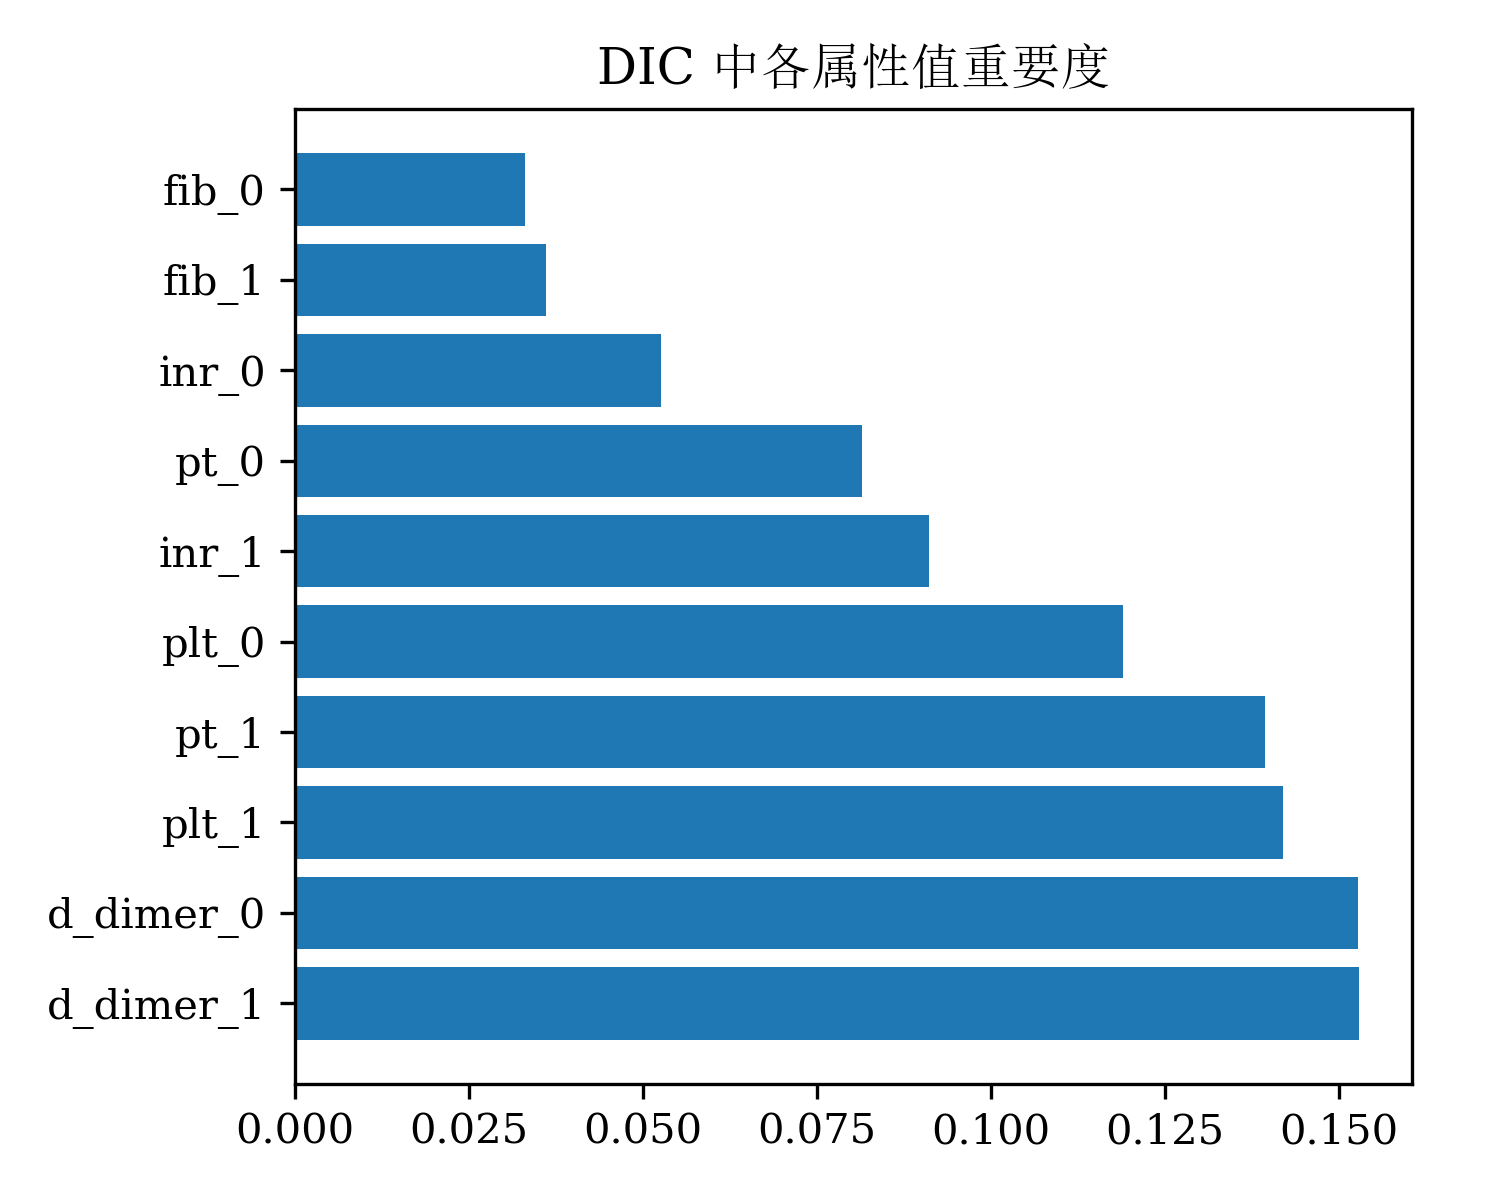
\includegraphics[scale=0.8]{dic_attributes_rank.png}
        \end{minipage}
    }
    \subfigure
    {
        \begin{minipage}[b]{.2\linewidth}
            \centering
            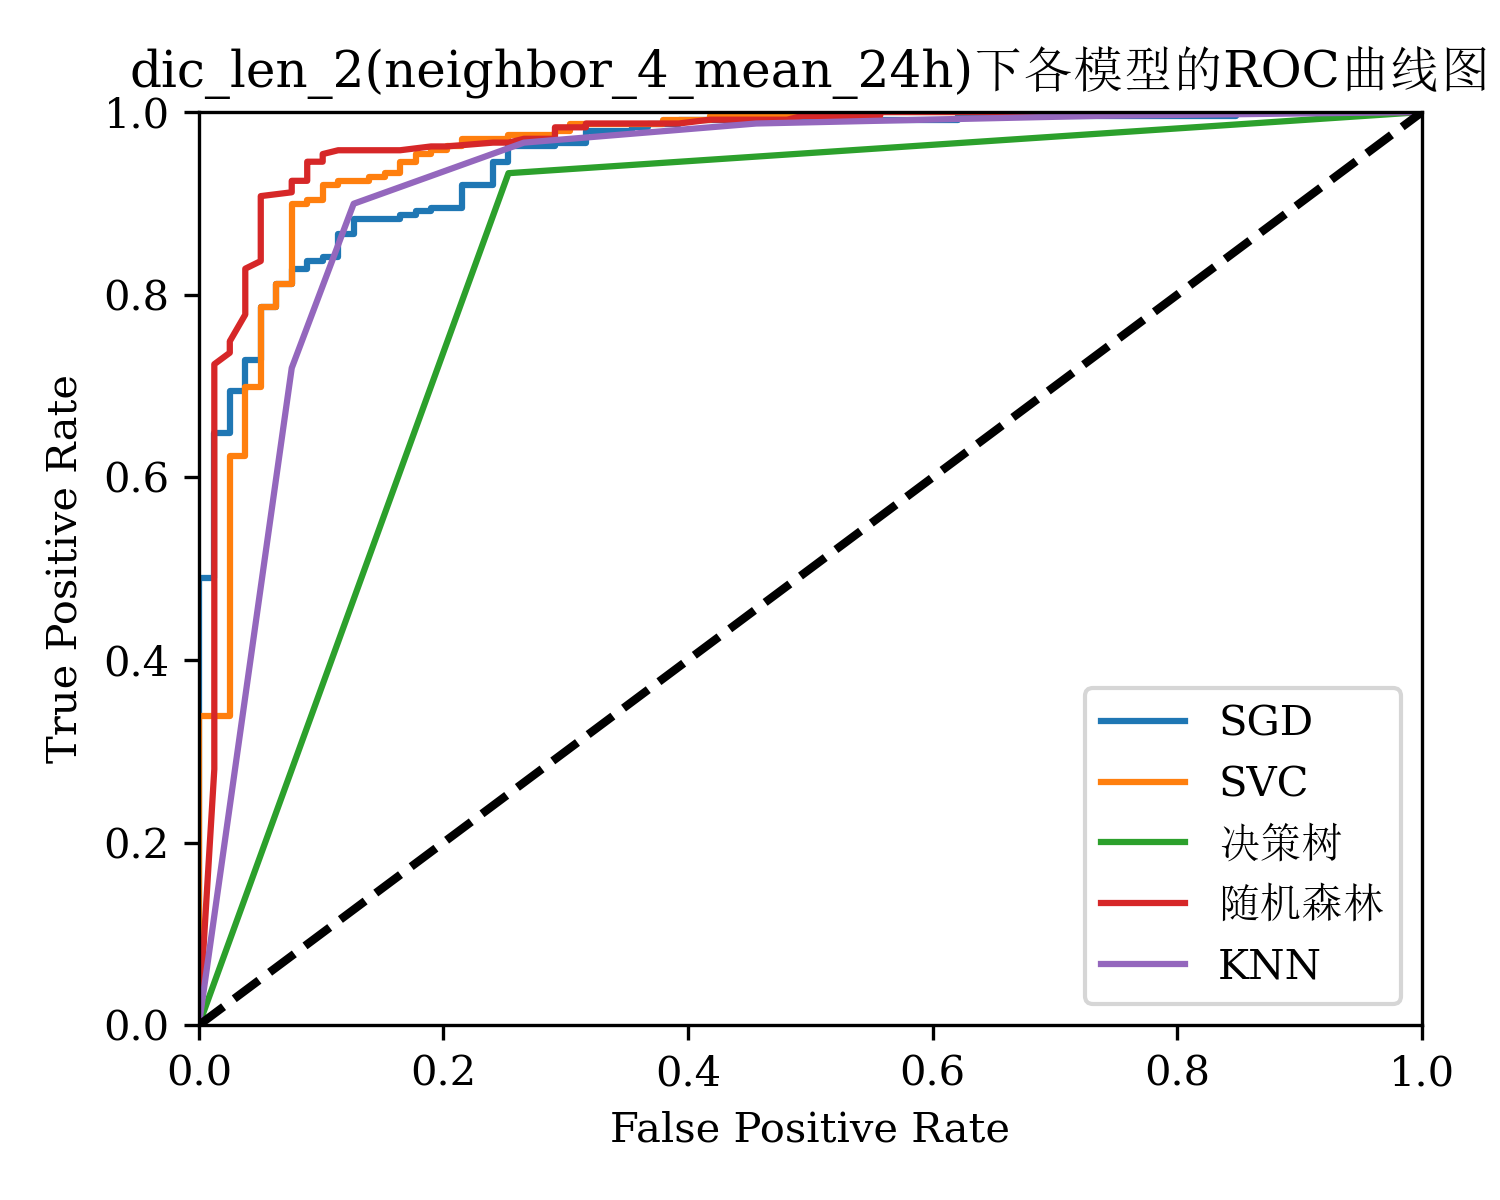
\includegraphics[scale=0.8]{dic_len_2(neighbor_4_mean_24h)_roc_curves.png}
        \end{minipage}
    }
\end{figure}
\begin{figure}[htbp]
    \centering
    \caption{DIC重要度分布}
\end{figure}
\section{结论与展望}
\clearpage
\begin{thebibliography}{99}
    \bibitem{ref1} 你好
\end{thebibliography}
\clearpage
\appendix
\section{附录}
\end{document}
